\part{Robot Operating System 2 (ROS 2)}

\begin{frame}{References}
    \begin{columns}[c]
        \begin{column}{.45\textwidth}
            \begin{figure}
                \centering
                
\includegraphics[scale=0.15]{img/ros2/ros2_logo.jpeg}
                
\includegraphics[scale=0.15]{img/ros2/ros2_humble.png}
            \end{figure}
        \end{column}
        \begin{column}{.45\textwidth}
            \centering
            \small
            \href{https://docs.ros.org/en/humble/}{ROS 2 Documentation}

            \vspace{0.3cm}

            \href{https://www.ros.org/}{ROS 2 Official Website}

            \vspace{0.3cm}

            \href{https://github.com/ros2/ros2_documentation}{ROS 2 Tutorials}
        \end{column}
    \end{columns}
\end{frame}

\section{Introduction to ROS 2}

\begin{frame}{What is ROS?}
    \begin{block}{Definition}
        \textbf{ROS (Robot Operating System)} is an open-source, flexible framework for writing robot software.
        \begin{itemize}
            \item Not an actual operating system, but a \textbf{middleware}
            \item Collection of tools, libraries, and conventions
            \item Facilitates communication between processes
            \item Provides hardware abstraction and low-level device control
        \end{itemize}
    \end{block}

    \begin{block}{Key Features}
        \begin{itemize}
            \item \textbf{Distributed computing}: Processes can run on multiple machines
            \item \textbf{Reusable code}: Extensive package ecosystem
            \item \textbf{Language independence}: C++, Python, and more
            \item \textbf{Tool ecosystem}: Visualization, simulation, debugging
        \end{itemize}
    \end{block}
\end{frame}

\begin{frame}[allowframebreaks]{History and Motivation}
    \begin{block}{The Problem Before ROS}
        \begin{itemize}
            \item Robot development required \textbf{reinventing the wheel}
            \item No standardized way to share code between robots
            \item Difficult to integrate different hardware and sensors
            \item Limited collaboration across research groups
            \item Each project started from scratch
        \end{itemize}
    \end{block}

    \framebreak

    \begin{block}{ROS History}
        \begin{itemize}
            \item \textbf{2007}: Started at Stanford University (STAIR project)
            \item \textbf{2008}: Development continued at Willow Garage
            \item \textbf{2010}: ROS 1.0 released
            \item \textbf{2013}: Open Source Robotics Foundation (OSRF) created
            \item \textbf{2017}: ROS 2 development begins in earnest
            \item \textbf{2020}: ROS 2 reaches production maturity
            \item \textbf{Today}: Used worldwide in research, industry, and education
        \end{itemize}
    \end{block}

    \framebreak

    \begin{block}{Why ROS Succeeded}
        \begin{itemize}
            \item \textbf{Open source}: Free to use and modify
            \item \textbf{Community-driven}: Thousands of contributors
            \item \textbf{Rich ecosystem}: Thousands of packages available
            \item \textbf{Industry adoption}: Used in commercial robots
            \item \textbf{Educational value}: Widely taught in universities
            \item \textbf{Active development}: Continuous improvements
        \end{itemize}
    \end{block}

    \begin{alertblock}{ROS Versions}
        \textbf{ROS 1}: Mature, widely used, but with limitations\\
        \textbf{ROS 2}: Modern redesign addressing ROS 1 limitations
    \end{alertblock}
\end{frame}

\begin{frame}[allowframebreaks]{Why ROS 2? }
    \begin{block}{Limitations of ROS 1}
        \begin{itemize}
            \item \textbf{Single point of failure}: roscore required for all communications
            \item \textbf{No real-time support}: not suitable for safety-critical systems
            \item \textbf{Limited multi-robot support}: challenging to run multiple robots
            \item \textbf{Network dependency}: relies heavily on stable network connections
            \item \textbf{Security}: minimal built-in security features
            \item \textbf{Platform support}: primarily Linux-focused
        \end{itemize}
    \end{block}

    \framebreak

    \begin{block}{ROS 2 Improvements}
        \begin{itemize}
            \item \textbf{No roscore}: fully distributed peer-to-peer architecture
            \item \textbf{Real-time capable}: support for real-time systems with DDS
            \item \textbf{Multi-robot native}: designed for multiple robot systems
            \item \textbf{Better reliability}: no single point of failure
            \item \textbf{Security}: built-in security features (SROS2)
            \item \textbf{Cross-platform}: Windows, Linux, and macOS support
            \item \textbf{Production ready}: suitable for commercial products
        \end{itemize}
    \end{block}
\end{frame}

\begin{frame}{ROS 2 Architecture}

    \begin{itemize}
        \item Built on top of \textbf{DDS} (Data Distribution Service)
        \item DDS provides \textbf{discovery}, \textbf{serialization}, and \textbf{transportation}
        \item Multiple DDS implementations supported (FastDDS, CycloneDDS, etc.)
    \end{itemize}
    \begin{figure}
        \centering
        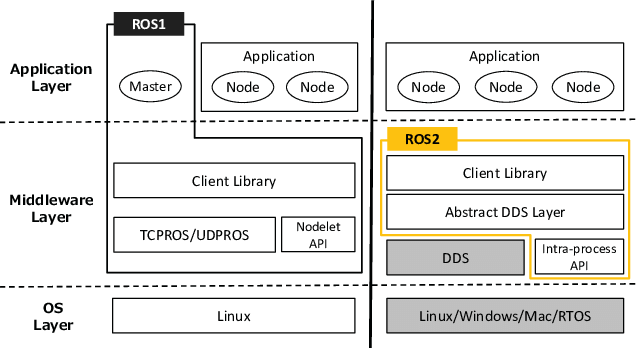
\includegraphics[width=0.99\textheight]{img/ros2/ROS1-ROS2-architecture-1.png}
        \caption{ROS 2 Architecture based on DDS}
    \end{figure}
\end{frame}

\begin{frame}[allowframebreaks]{What is DDS?}
    \begin{block}{Definition}
        \textbf{DDS (Data Distribution Service)} is an industry-standard protocol for real-time, scalable, and high-performance data exchange.
        \begin{itemize}
            \item Standardized by \textbf{Object Management Group (OMG)}
            \item Publish-subscribe middleware for distributed systems
            \item Used in mission-critical applications (aerospace, defense, healthcare)
        \end{itemize}
    \end{block}

    \framebreak

    \begin{block}{Key Features of DDS}
        \begin{itemize}
            \item \textbf{Decentralized}: No central broker required (peer-to-peer)
            \item \textbf{Quality of Service (QoS)}: Fine-grained control over reliability, latency, bandwidth
            \item \textbf{Data-centric}: Focus on data rather than connections
            \item \textbf{Discovery}: Automatic discovery of publishers and subscribers
            \item \textbf{Real-time capable}: Deterministic and low-latency communication
            \item \textbf{Scalable}: Supports large-scale distributed systems
        \end{itemize}
    \end{block}

    \framebreak

    \begin{block}{DDS Implementations in ROS 2}
        ROS 2 supports multiple DDS vendors:
        \begin{itemize}
            \item \textbf{Fast DDS} (eProsima): Default in ROS 2 Humble
            \item \textbf{Cyclone DDS} (Eclipse Foundation): Lightweight and fast
        \end{itemize}
    \end{block}

    \begin{alertblock}{Why DDS for ROS 2?}
        DDS solves ROS 1 limitations: no single point of failure, built-in QoS, real-time support, and production-ready reliability.
    \end{alertblock}
\end{frame}

\begin{frame}[allowframebreaks]{ROS 2 Distributions}
    \begin{block}{LTS (Long Term Support) Distributions}
        \begin{itemize}
            \item \textbf{Humble Hawksbill} (May 2022): Ubuntu 22.04, supported until May 2027
            \item \textbf{Foxy Fitzroy} (June 2020): Ubuntu 20.04, supported until May 2023
        \end{itemize}
    \end{block}

    \begin{block}{Current Distributions (as of 2024)}
        \begin{itemize}
            \item \textbf{Iron Irwini} (May 2023): Ubuntu 22.04
            \item \textbf{Jazzy Jalisco} (May 2024): Ubuntu 24.04
            \item Rolling Ridley: continuously updated development distribution
        \end{itemize}
    \end{block}

    \begin{alertblock}{Recommendation}
        For production and learning, use \textbf{Humble Hawksbill} (LTS version)
    \end{alertblock}
\end{frame}

\section{ROS 2 Concepts}

\begin{frame}[allowframebreaks]{ROS 2 Core Concepts}
    \begin{description}[leftmargin=3cm]
        \item[Nodes] Processes that perform computation. Same as ROS 1 but with improved lifecycle management.

        \item[Topics] Named buses for asynchronous communication using publish/subscribe pattern. Similar to ROS 1.

        \item[Services] Synchronous request-reply communication. Enhanced in ROS 2 with better timeout handling.

        \item[Actions] Asynchronous goal-oriented tasks with feedback. Improved implementation compared to ROS 1.

        \item[Parameters] Runtime configuration values for nodes. Enhanced with parameter events and better type safety.

        \item[Quality of Service (QoS)] NEW in ROS 2: fine-grained control over communication behavior (reliability, durability, etc.).
    \end{description}
\end{frame}

\begin{frame}{ROS 2 Communication: Topics}
    \begin{block}{Definition}
        Buses \textbf{many-to-many}, \textbf{asynchronous} communication using the publish-subscribe pattern.
        \begin{itemize}
            \item Multiple publishers/subscribers can send/receive messages to/from a topic
            \item Fire-and-forget: publishers don't wait for acknowledgment
            \item Best for: sensor data, continuous streams (e.g., camera images, laser scans)
        \end{itemize}
    \end{block}

    \begin{figure}
        \centering
        \href{https://docs.ros.org/en/foxy/Tutorials/Beginner-CLI-Tools/Understanding-ROS2-Topics/Understanding-ROS2-Topics.html}{%
            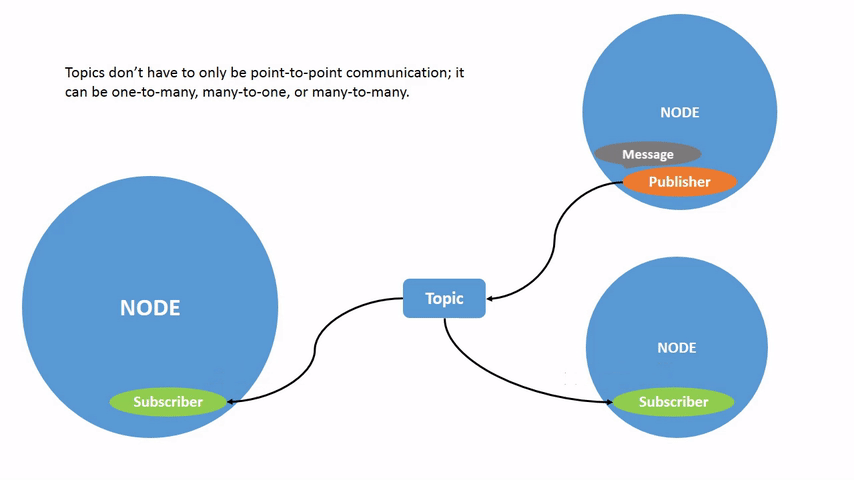
\includegraphics[width=0.5\textwidth]{img/ros2/ros2_communication.png}%
        }
        \caption{Topic communication pattern (click for tutorial)}
    \end{figure}
\end{frame}

\begin{frame}{ROS 2 Communication: Services}
    \begin{block}{Definition}
        Provide \textbf{one-to-one}, \textbf{synchronous} request-reply communication.
        \small
        \begin{itemize}
            \item Client sends a request and waits for response
            \item Server processes the request and sends back a reply
            \item Blocking operation: client waits for the response
            \item Best for: occasional tasks, computations (e.g., inverse kinematics, spawn entities)
        \end{itemize}
    \end{block}

    \begin{figure}
        \centering
        \href{https://docs.ros.org/en/foxy/Tutorials/Beginner-CLI-Tools/Understanding-ROS2-Services/Understanding-ROS2-Services.html}{%
            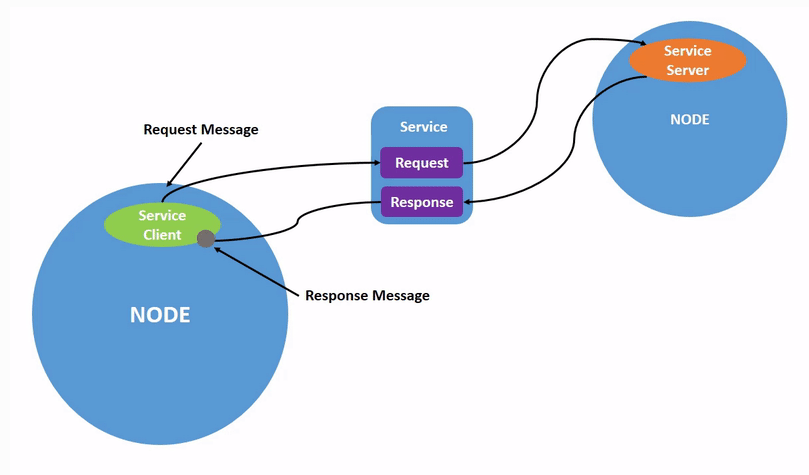
\includegraphics[width=0.5\textwidth]{img/ros2/ros2_communication_service.png}%
        }
        \caption{Service communication pattern (click for tutorial)}
    \end{figure}
\end{frame}

\begin{frame}{ROS 2 Communication: Actions}
    \begin{block}{Definition}
        Designed for \textbf{asynchronous}, \textbf{long-running} tasks with feedback and the ability to cancel.
        \begin{itemize}
            \item Client sends a goal and receives periodic feedback
            \item Server can send progress updates while executing
            \item Goals can be cancelled by the client
            \item Result is sent when the action completes
            \item Best for: navigation, manipulation, time-consuming operations
        \end{itemize}
    \end{block}

    \begin{figure}
        \centering
        \href{https://docs.ros.org/en/foxy/Tutorials/Beginner-CLI-Tools/Understanding-ROS2-Actions/Understanding-ROS2-Actions.html}{%
            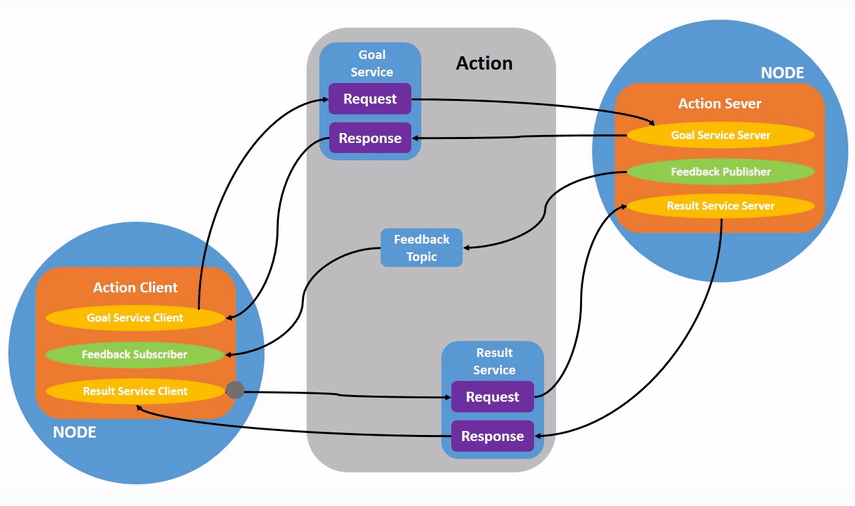
\includegraphics[width=0.3\textwidth]{img/ros2/ros2_communication_actions.png}%
        }
        \caption{Action communication pattern (click for tutorial)}
    \end{figure}
\end{frame}

\section{Installing ROS 2}

\begin{frame}[fragile, allowframebreaks]{Ubuntu install of ROS 2 Humble}
    ROS 2 Humble supports Ubuntu 22.04 (Jammy Jellyfish).

    \href{https://docs.ros.org/en/humble/Installation/Ubuntu-Install-Debs.html}{Installation instructions}

    \begin{enumerate}
        \item \textbf{Set locale}:
              \begin{lstlisting}[language=shell]
$ locale  # check for UTF-8
$ sudo apt update && sudo apt install locales
$ sudo locale-gen en_US en_US.UTF-8
$ sudo update-locale LC_ALL=en_US.UTF-8 LANG=en_US.UTF-8
$ export LANG=en_US.UTF-8
\end{lstlisting}

        \item \textbf{Setup Sources}:
              \begin{lstlisting}[language=shell]
$ sudo apt install software-properties-common
$ sudo add-apt-repository universe
$ sudo apt update && sudo apt install curl -y
$ sudo curl -sSL https://raw.githubusercontent.com/ros/rosdistro/master/ros.key -o /usr/share/keyrings/ros-archive-keyring.gpg
\end{lstlisting}

              \framebreak

              \begin{lstlisting}[language=shell]
$ echo "deb [arch=$(dpkg --print-architecture) signed-by=/usr/share/keyrings/ros-archive-keyring.gpg] http://packages.ros.org/ros2/ubuntu $(. /etc/os-release && echo $UBUNTU_CODENAME) main" | sudo tee /etc/apt/sources.list.d/ros2.list > /dev/null
\end{lstlisting}

        \item \textbf{Install ROS 2 packages}:
              \begin{lstlisting}[language=shell]
$ sudo apt update
$ sudo apt upgrade
$ sudo apt install ros-humble-desktop
\end{lstlisting}

        \item \textbf{Environment setup}:
              \begin{lstlisting}[language=shell]
$ source /opt/ros/humble/setup.bash
$ echo "source /opt/ros/humble/setup.bash" >> ~/.bashrc
\end{lstlisting}

        \item \textbf{Install development tools}:
              \begin{lstlisting}[language=shell]
$ sudo apt install ros-dev-tools
\end{lstlisting}
    \end{enumerate}
\end{frame}

\begin{frame}[fragile, allowframebreaks]{Setting up Docker image for ROS 2}
    \begin{enumerate}
        \item \textbf{Download the image from Docker Hub}:
              \begin{lstlisting}[language=shell]
$ docker pull osrf/ros:humble-desktop-full
\end{lstlisting}

        \item \textbf{Launch the container using Rocker}:
              \begin{lstlisting}[language=shell]
$ rocker --nvidia --x11 --network host --name ros2-humble --volume <path_to_shared_folder>:/root/ros2_ws -- docker.io/osrf/ros:humble-desktop-full
\end{lstlisting}
              \textcolor{blue}{- -nvidia option only if the computer has a graphic card}\\
              \textcolor{blue}{- -volume for sharing folder between host and container}

        \item \textbf{To open a new terminal inside the container}:
              \begin{lstlisting}[language=shell]
$ docker exec -it ros2-humble /bin/bash 
\end{lstlisting}

              \framebreak

        \item \textbf{To source the ROS 2 environment}:
              \begin{lstlisting}[language=shell]
$ source /opt/ros/humble/setup.bash
\end{lstlisting}

        \item \textbf{To source the workspace} (after building):
              \begin{lstlisting}[language=shell]
$ source /root/ros2_ws/install/setup.bash
\end{lstlisting}
    \end{enumerate}
\end{frame}

\begin{frame}[fragile]{Verify Installation}
    Test that ROS 2 is installed correctly:

    \begin{lstlisting}[language=shell]
$ ros2 --help
\end{lstlisting}

    You should see a list of available commands:
    \begin{lstlisting}[language=output]
usage: ros2 [-h] Call `ros2 <command> -h` for more detailed usage. ...

ros2 is an extensible command-line tool for ROS 2.
  ...
\end{lstlisting}

    \framebreak

    Main commands:
    \begin{lstlisting}[language=syntax]
ros2 node      # Node introspection tools
ros2 topic     # Topic introspection tools
ros2 service   # Service introspection tools
ros2 action    # Action introspection tools
ros2 param     # Parameter introspection tools
ros2 bag       # Recording and playback tools
ros2 run       # Run a node
ros2 launch    # Launch files
ros2 pkg       # Package tools
ros2 interface # Interface introspection
\end{lstlisting}
\end{frame}

\section{ROS 2 Workspace}

\begin{frame}[fragile, allowframebreaks]{Creating a ROS 2 Workspace}
    A ROS 2 workspace is organized differently from ROS 1:

    \begin{lstlisting}[language=shell]
$ mkdir -p ~/ros2_ws/src
$ cd ~/ros2_ws
\end{lstlisting}

    \textbf{Build the workspace} using colcon (Inside the ros2\_ws directory):
    \begin{lstlisting}[language=shell]
$ colcon build
\end{lstlisting}

    After building, you'll have these directories:
    \begin{lstlisting}[language=syntax]
ros2_ws/
  build/    # Build artifacts
  install/  # Installation files
  log/      # Build logs
  src/      # Source code
\end{lstlisting}

    \framebreak

    \textbf{Source the workspace}:
    \begin{lstlisting}[language=shell]
$ source ~/ros2_ws/install/setup.bash
\end{lstlisting}

    To automatically source on every new terminal:
    \begin{lstlisting}[language=shell]
$ echo "source ~/ros2_ws/install/setup.bash" >> ~/.bashrc
\end{lstlisting}

    \begin{alertblock}{Build specific packages}
        \begin{lstlisting}[language=shell]
$ colcon build --packages-select <package_name>
\end{lstlisting}
    \end{alertblock}
\end{frame}

\begin{frame}[fragile]{Installing Turtlesim}
    \textbf{Turtlesim} is a lightweight simulator for learning ROS 2 concepts.
    \\ \href{https://docs.ros.org/en/humble/Tutorials/Beginner-CLI-Tools/Introducing-Turtlesim/Introducing-Turtlesim.html}{Learn more about Turtlesim.}

    \begin{block}{Install on Ubuntu}
        \begin{lstlisting}[language=shell]
$ sudo apt update
$ sudo apt install ros-humble-turtlesim
\end{lstlisting}
    \end{block}

    \begin{block}{Verify installation}
        Check if turtlesim package is available:
        \begin{lstlisting}[language=shell]
$ ros2 pkg executables turtlesim
turtlesim draw_square
turtlesim mimic
turtlesim turtle_teleop_key
turtlesim turtlesim_node
\end{lstlisting}
    \end{block}
\end{frame}

\begin{frame}[fragile]{Running Turtlesim}
    \textbf{Start the turtlesim node}:
    \begin{lstlisting}[language=shell]
$ ros2 run turtlesim turtlesim_node
\end{lstlisting}

    A window will appear with a turtle in the center.

    \vspace{0.5cm}

    \textbf{In a new terminal, start the teleop node}:
    \begin{lstlisting}[language=shell]
$ ros2 run turtlesim turtle_teleop_key
\end{lstlisting}

    Use arrow keys to control the turtle!

    \begin{alertblock}{Tip}
        Make sure the terminal with \texttt{turtle\_teleop\_key} is active (in focus) when pressing arrow keys.
    \end{alertblock}
\end{frame}

\begin{frame}[fragile]{Turtlesim in Docker}
    If running ROS 2 in Docker, you need X11 forwarding for GUI applications.

    \begin{block}{Using Rocker (recommended)}
        \begin{lstlisting}[language=shell]
$ rocker --x11 --nvidia osrf/ros:humble-desktop-full
\end{lstlisting}
    \end{block}

    \begin{block}{Inside the container}
        \begin{lstlisting}[language=shell]
$ source /opt/ros/humble/setup.bash
$ apt update && apt install -y ros-humble-turtlesim
$ ros2 run turtlesim turtlesim_node
\end{lstlisting}
    \end{block}

    \begin{alertblock}{Note}
        The \texttt{--x11} flag enables X11 forwarding for displaying GUI windows.
    \end{alertblock}
\end{frame}

\begin{frame}[fragile, allowframebreaks]{Working with Nodes}
    \textbf{List running nodes}:
    \begin{lstlisting}[language=shell]
$ ros2 node list
\end{lstlisting}

    \textbf{Get node information}:
    \begin{lstlisting}[language=shell]
$ ros2 node info /node_name
\end{lstlisting}

    \textbf{Run a node}:
    \begin{lstlisting}[language=shell]
$ ros2 run <package_name> <executable_name>
\end{lstlisting}

    Example with turtlesim:
    \begin{lstlisting}[language=shell]
$ sudo apt install ros-humble-turtlesim
$ ros2 run turtlesim turtlesim_node
\end{lstlisting}

    \framebreak

    \textbf{Remap node name}:
    \begin{lstlisting}[language=shell]
$ ros2 run turtlesim turtlesim_node --ros-args --remap __node:=my_turtle
\end{lstlisting}

    \textbf{Get node info}:
    \begin{lstlisting}[language=shell]
$ ros2 node info /turtlesim
Node [/turtlesim]
  Subscribers:
    /turtle1/cmd_vel: geometry_msgs/msg/Twist
  Publishers:
    /turtle1/color_sensor: turtlesim/msg/Color
    /turtle1/pose: turtlesim/msg/Pose
  Service Servers:
    /clear: std_srvs/srv/Empty
    /kill: turtlesim/srv/Kill
    ...
\end{lstlisting}
\end{frame}

\begin{frame}[fragile, allowframebreaks]{Working with Topics}
    \textbf{List topics}:
    \begin{lstlisting}[language=shell]
$ ros2 topic list
$ ros2 topic list -t  # Show message types
\end{lstlisting}

    \textbf{Echo topic messages}:
    \begin{lstlisting}[language=shell]
$ ros2 topic echo /turtle1/cmd_vel
\end{lstlisting}

    \textbf{Get topic info}:
    \begin{lstlisting}[language=shell]
$ ros2 topic info /turtle1/cmd_vel
Type: geometry_msgs/msg/Twist
Publisher count: 1
Subscription count: 1
\end{lstlisting}

    \framebreak

    \textbf{Publish to a topic}:
    \begin{lstlisting}[language=shell]
$ ros2 topic pub /turtle1/cmd_vel geometry_msgs/msg/Twist "{linear: {x: 2.0, y: 0.0, z: 0.0}, angular: {x: 0.0, y: 0.0, z: 1.8}}"
\end{lstlisting}

    Add \texttt{--once} to publish once or \texttt{--rate 1} for continuous publishing at 1 Hz.

    \textbf{Get publishing frequency}:
    \begin{lstlisting}[language=shell]
$ ros2 topic hz /turtle1/pose
average rate: 62.506
	min: 0.014s max: 0.018s std dev: 0.00070s window: 64
\end{lstlisting}

    \textbf{Get bandwidth}:
    \begin{lstlisting}[language=shell]
$ ros2 topic bw /turtle1/pose
\end{lstlisting}
\end{frame}

\begin{frame}[fragile, allowframebreaks]{Working with Services}
    \textbf{List services}:
    \begin{lstlisting}[language=shell]
$ ros2 service list
$ ros2 service list -t  # Show service types
\end{lstlisting}

    \textbf{Get service type}:
    \begin{lstlisting}[language=shell]
$ ros2 service type /clear
std_srvs/srv/Empty
\end{lstlisting}

    \textbf{Find services by type}:
    \begin{lstlisting}[language=shell]
$ ros2 service find std_srvs/srv/Empty
/clear
/reset
\end{lstlisting}

    \framebreak

    \textbf{Call a service}:
    \begin{lstlisting}[language=shell]
$ ros2 service call /clear std_srvs/srv/Empty
\end{lstlisting}

    Spawn a new turtle:
    \begin{lstlisting}[language=shell]
$ ros2 service call /spawn turtlesim/srv/Spawn "{x: 2.0, y: 2.0, theta: 0.2, name: 'turtle2'}"
\end{lstlisting}

    \textbf{Show service interface}:
    \begin{lstlisting}[language=shell]
$ ros2 interface show turtlesim/srv/Spawn
float32 x
float32 y
float32 theta
string name
---
string name
\end{lstlisting}
\end{frame}

\begin{frame}[fragile, allowframebreaks]{Working with Parameters}
    \textbf{List parameters}:
    \begin{lstlisting}[language=shell]
$ ros2 param list
\end{lstlisting}

    \textbf{Get parameter value}:
    \begin{lstlisting}[language=shell]
$ ros2 param get /turtlesim background_r
Integer value is: 69
\end{lstlisting}

    \textbf{Set parameter value}:
    \begin{lstlisting}[language=shell]
$ ros2 param set /turtlesim background_r 150
Set parameter successful
\end{lstlisting}

    \framebreak

    \textbf{Dump parameters to file}:
    \begin{lstlisting}[language=shell]
$ ros2 param dump /turtlesim
Saving to:  ./turtlesim.yaml
\end{lstlisting}

    \textbf{Load parameters from file}:
    \begin{lstlisting}[language=shell]
$ ros2 param load /turtlesim turtlesim.yaml
\end{lstlisting}

    \textbf{Start node with parameters}:
    \begin{lstlisting}[language=shell]
$ ros2 run turtlesim turtlesim_node --ros-args --params-file turtlesim.yaml
\end{lstlisting}
\end{frame}

\begin{frame}[fragile, allowframebreaks]{Working with Actions}
    Actions are for long-running tasks with feedback.

    \textbf{List actions}:
    \begin{lstlisting}[language=shell]
$ ros2 action list
$ ros2 action list -t  # Show action types
\end{lstlisting}

    \textbf{Get action info}:
    \begin{lstlisting}[language=shell]
$ ros2 action info /turtle1/rotate_absolute
Action: /turtle1/rotate_absolute
Action clients: 0
Action servers: 1
    /turtlesim
\end{lstlisting}

    \framebreak

    \textbf{Show action interface}:
    \begin{lstlisting}[language=shell]
$ ros2 interface show turtlesim/action/RotateAbsolute
# Goal
float32 theta
---
# Result
float32 delta
---
# Feedback
float32 remaining
\end{lstlisting}

    \textbf{Send action goal}:
    \begin{lstlisting}[language=shell]
$ ros2 action send_goal /turtle1/rotate_absolute turtlesim/action/RotateAbsolute "{theta: 1.57}" --feedback
\end{lstlisting}
\end{frame}

\section{Creating ROS 2 Packages}

\begin{frame}[fragile, allowframebreaks]{Creating a Package}
    ROS 2 supports two build types: \textbf{ament\_cmake} and \textbf{ament\_python}.

    \textbf{Create a Python package}:
    \begin{lstlisting}[language=shell]
$ cd ~/ros2_ws/src
$ ros2 pkg create --build-type ament_python --node-name my_node my_package
\end{lstlisting}

    \textbf{Create a C++ package}:
    \begin{lstlisting}[language=shell]
$ ros2 pkg create --build-type ament_cmake --node-name my_node my_package --dependencies rclcpp std_msgs
\end{lstlisting}

    \framebreak

    \textbf{Package structure} (Python):
    \begin{lstlisting}[language=syntax]
my_package/
  my_package/
    __init__.py
    my_node.py
  resource/
    my_package
  test/
  package.xml
  setup.py
  setup.cfg
\end{lstlisting}

    \framebreak

    \textbf{Package structure} (C++):
    \begin{lstlisting}[language=syntax]
my_package/
  include/
    my_package/
  src/
    my_node.cpp
  CMakeLists.txt
  package.xml
\end{lstlisting}
\end{frame}

\begin{frame}[fragile]{Building and Running}
    \textbf{Build the package}:
    \begin{lstlisting}[language=shell]
$ cd ~/ros2_ws
$ colcon build --packages-select my_package
\end{lstlisting}

    \textbf{Source the workspace}:
    \begin{lstlisting}[language=shell]
$ source ~/ros2_ws/install/setup.bash
\end{lstlisting}

    \textbf{Run the node}:
    \begin{lstlisting}[language=shell]
$ ros2 run my_package my_node
\end{lstlisting}

    \begin{alertblock}{Tip}
        Use \texttt{--symlink-install} flag for Python packages to avoid rebuilding after code changes:
        \begin{lstlisting}[language=shell]
$ colcon build --symlink-install
\end{lstlisting}
    \end{alertblock}
\end{frame}

\section{Writing Nodes in Python}

\begin{frame}[fragile, allowframebreaks]{Simple Publisher (Python)}
    Create file \texttt{publisher\_member\_function.py}:

    \begin{lstlisting}[language=python]
import rclpy
from rclpy.node import Node
from std_msgs.msg import String

class MinimalPublisher(Node):
    def __init__(self):
        super().__init__('minimal_publisher')
        self.publisher_ = self.create_publisher(String, 'topic', 10)
        timer_period = 0.5  # seconds
        self.timer = self.create_timer(timer_period, self.timer_callback)
        self.i = 0

    def timer_callback(self):
        msg = String()
        msg.data = 'Hello World: %d' % self.i
        self.publisher_.publish(msg)
        self.get_logger().info('Publishing: "%s"' % msg.data)
        self.i += 1

def main(args=None):
    rclpy.init(args=args)
    minimal_publisher = MinimalPublisher()
    rclpy.spin(minimal_publisher)
    minimal_publisher.destroy_node()
    rclpy.shutdown()

if __name__ == '__main__':
    main()
\end{lstlisting}

    \framebreak

    \textbf{Key concepts}:
    \begin{itemize}
        \item \texttt{rclpy.init()}: Initialize ROS 2 Python client library
        \item \texttt{Node}: Base class for ROS 2 nodes
        \item \texttt{create\_publisher()}: Create a publisher with topic name, message type, and QoS
        \item \texttt{create\_timer()}: Create a timer for periodic callbacks
        \item \texttt{rclpy.spin()}: Keep the node running
        \item \texttt{get\_logger()}: Built-in logging functionality
    \end{itemize}
\end{frame}

\begin{frame}[fragile, allowframebreaks]{Simple Subscriber (Python)}
    Create file \texttt{subscriber\_member\_function.py}:

    \begin{lstlisting}[language=python]
import rclpy
from rclpy.node import Node
from std_msgs.msg import String

class MinimalSubscriber(Node):
    def __init__(self):
        super().__init__('minimal_subscriber')
        self.subscription = self.create_subscription(
            String,
            'topic',
            self.listener_callback,
            10)
        self.subscription  # prevent unused variable warning

    def listener_callback(self, msg):
        self.get_logger().info('I heard: "%s"' % msg.data)

def main(args=None):
    rclpy.init(args=args)
    minimal_subscriber = MinimalSubscriber()
    rclpy.spin(minimal_subscriber)
    minimal_subscriber.destroy_node()
    rclpy.shutdown()

if __name__ == '__main__':
    main()
\end{lstlisting}

    \framebreak

    \textbf{Add to setup.py}:
    \begin{lstlisting}[language=python]
entry_points={
    'console_scripts': [
        'talker = my_package.publisher_member_function:main',
        'listener = my_package.subscriber_member_function:main',
    ],
},
\end{lstlisting}

    \textbf{Build and run}:
    \begin{lstlisting}[language=shell]
$ cd ~/ros2_ws
$ colcon build --packages-select my_package
$ source install/setup.bash
$ ros2 run my_package talker
\end{lstlisting}

    In another terminal:
    \begin{lstlisting}[language=shell]
$ ros2 run my_package listener
\end{lstlisting}
\end{frame}

\begin{frame}[fragile, allowframebreaks]{Service Server (Python)}
    Create file \texttt{service\_member\_function.py}:

    \begin{lstlisting}[language=python]
from example_interfaces.srv import AddTwoInts
import rclpy
from rclpy.node import Node

class MinimalService(Node):
    def __init__(self):
        super().__init__('minimal_service')
        self.srv = self.create_service(
            AddTwoInts, 
            'add_two_ints', 
            self.add_two_ints_callback)

    def add_two_ints_callback(self, request, response):
        response.sum = request.a + request.b
        self.get_logger().info(
            'Incoming request\na: %d b: %d' % (request.a, request.b))
        return response

def main(args=None):
    rclpy.init(args=args)
    minimal_service = MinimalService()
    rclpy.spin(minimal_service)
    rclpy.shutdown()

if __name__ == '__main__':
    main()
\end{lstlisting}
\end{frame}

\begin{frame}[fragile, allowframebreaks]{Service Client (Python)}
    Create file \texttt{client\_member\_function.py}:

    \begin{lstlisting}[language=python]
import sys
from example_interfaces.srv import AddTwoInts
import rclpy
from rclpy.node import Node

class MinimalClientAsync(Node):
    def __init__(self):
        super().__init__('minimal_client_async')
        self.cli = self.create_client(AddTwoInts, 'add_two_ints')
        while not self.cli.wait_for_service(timeout_sec=1.0):
            self.get_logger().info('service not available, waiting...')
        self.req = AddTwoInts.Request()

    def send_request(self, a, b):
        self.req.a = a
        self.req.b = b
        self.future = self.cli.call_async(self.req)
        rclpy.spin_until_future_complete(self, self.future)
        return self.future.result()

def main(args=None):
    rclpy.init(args=args)
    minimal_client = MinimalClientAsync()
    response = minimal_client.send_request(int(sys.argv[1]), int(sys.argv[2]))
    minimal_client.get_logger().info(
        'Result of add_two_ints: %d + %d = %d' %
        (int(sys.argv[1]), int(sys.argv[2]), response.sum))
    minimal_client.destroy_node()
    rclpy.shutdown()

if __name__ == '__main__':
    main()
\end{lstlisting}
\end{frame}

\section{Launch Files}

\begin{frame}[fragile, allowframebreaks]{ROS 2 Launch Files}
    Launch files in ROS 2 can be written in \textbf{Python}, XML, or YAML.

    \textbf{Python launch file} (\texttt{my\_launch.py}):
    \begin{lstlisting}[language=python]
from launch import LaunchDescription
from launch_ros.actions import Node

def generate_launch_description():
    return LaunchDescription([
        Node(
            package='turtlesim',
            executable='turtlesim_node',
            name='sim'
        ),
        Node(
            package='turtlesim',
            executable='turtle_teleop_key',
            name='teleop',
            prefix='xterm -e',
            output='screen'
        ),
    ])
\end{lstlisting}

    \framebreak

    \textbf{Create launch directory}:
    \begin{lstlisting}[language=shell]
$ mkdir -p ~/ros2_ws/src/my_package/launch
\end{lstlisting}

    \textbf{Update setup.py} to include launch files:
    \begin{lstlisting}[language=python]
import os
from glob import glob
# ...

data_files=[
    # ...
    (os.path.join('share', package_name, 'launch'), 
     glob('launch/*.py')),
],
\end{lstlisting}

    \framebreak

    \textbf{Run launch file}:
    \begin{lstlisting}[language=shell]
$ ros2 launch my_package my_launch.py
\end{lstlisting}

    \textbf{Launch with arguments}:
    \begin{lstlisting}[language=python]
from launch.actions import DeclareLaunchArgument
from launch.substitutions import LaunchConfiguration

def generate_launch_description():
    return LaunchDescription([
        DeclareLaunchArgument('use_sim_time', default_value='false'),
        Node(
            package='my_package',
            executable='my_node',
            parameters=[{'use_sim_time': LaunchConfiguration('use_sim_time')}]
        ),
    ])
\end{lstlisting}

    \begin{lstlisting}[language=shell]
$ ros2 launch my_package my_launch.py use_sim_time:=true
\end{lstlisting}
\end{frame}

\section{Custom Interfaces}

\begin{frame}[fragile, allowframebreaks]{Creating Custom Messages}
    \textbf{Create interface package}:
    \begin{lstlisting}[language=shell]
$ ros2 pkg create --build-type ament_cmake tutorial_interfaces
\end{lstlisting}

    \textbf{Create directory structure}:
    \begin{lstlisting}[language=shell]
$ mkdir -p tutorial_interfaces/msg
$ mkdir -p tutorial_interfaces/srv
$ mkdir -p tutorial_interfaces/action
\end{lstlisting}

    \textbf{Create custom message} (\texttt{msg/Num.msg}):
    \begin{lstlisting}[language=syntax]
int64 num
\end{lstlisting}

    \textbf{Create custom message with nested types} (\texttt{msg/Sphere.msg}):
    \begin{lstlisting}[language=syntax]
geometry_msgs/Point center
float64 radius
\end{lstlisting}

    \framebreak

    \textbf{Update CMakeLists.txt}:
    \begin{lstlisting}[language=syntax]
find_package(geometry_msgs REQUIRED)
find_package(rosidl_default_generators REQUIRED)

rosidl_generate_interfaces(${PROJECT_NAME}
  "msg/Num.msg"
  "msg/Sphere.msg"
  DEPENDENCIES geometry_msgs
)
\end{lstlisting}

    \textbf{Update package.xml}:
    \begin{lstlisting}[language=xml]
<depend>geometry_msgs</depend>
<buildtool_depend>rosidl_default_generators</buildtool_depend>
<exec_depend>rosidl_default_runtime</exec_depend>
<member_of_group>rosidl_interface_packages</member_of_group>
\end{lstlisting}

    \framebreak

    \textbf{Build the interface package}:
    \begin{lstlisting}[language=shell]
$ cd ~/ros2_ws
$ colcon build --packages-select tutorial_interfaces
$ source install/setup.bash
\end{lstlisting}

    \textbf{Verify the interface}:
    \begin{lstlisting}[language=shell]
$ ros2 interface show tutorial_interfaces/msg/Num
int64 num
\end{lstlisting}

    \textbf{Use in your node}:
    \begin{lstlisting}[language=python]
from tutorial_interfaces.msg import Num

# In your node:
self.publisher_ = self.create_publisher(Num, 'topic', 10)
msg = Num()
msg.num = 42
\end{lstlisting}
\end{frame}

\begin{frame}[fragile, allowframebreaks]{Creating Custom Services}
    \textbf{Create service definition} (\texttt{srv/AddThreeInts.srv}):
    \begin{lstlisting}[language=syntax]
int64 a
int64 b
int64 c
---
int64 sum
\end{lstlisting}

    \textbf{Update CMakeLists.txt}:
    \begin{lstlisting}[language=syntax]
rosidl_generate_interfaces(${PROJECT_NAME}
  "msg/Num.msg"
  "srv/AddThreeInts.srv"
)
\end{lstlisting}

    Build and verify:
    \begin{lstlisting}[language=shell]
$ colcon build --packages-select tutorial_interfaces
$ ros2 interface show tutorial_interfaces/srv/AddThreeInts
\end{lstlisting}
\end{frame}


\begin{frame}[allowframebreaks]{Quality of Service (QoS)}
    \begin{block}{What is QoS?}
        Quality of Service policies allow you to configure the behavior of communication in ROS 2:
        \begin{itemize}
            \item \textbf{Reliability}: Reliable (guaranteed delivery) vs Best Effort
            \item \textbf{Durability}: Transient Local (late joiners get last message) vs Volatile
            \item \textbf{History}: Keep Last N messages vs Keep All
            \item \textbf{Deadline}: Maximum time between messages
            \item \textbf{Lifespan}: Maximum age of a message
        \end{itemize}
    \end{block}

    \framebreak

    \begin{block}{QoS Profiles}
        ROS 2 provides predefined QoS profiles:
        \begin{itemize}
            \item \textbf{Sensor Data}: Best effort, volatile (e.g., camera images)
            \item \textbf{Parameters}: Reliable, volatile (e.g., configuration)
            \item \textbf{Services}: Reliable, volatile
            \item \textbf{System Default}: Reliable, volatile, keep last 10
        \end{itemize}
    \end{block}

    \begin{alertblock}{Important}
        Publishers and subscribers must have \textbf{compatible} QoS policies to communicate!
    \end{alertblock}
\end{frame}

\section{ROS 2 Tools and Visualization}

\begin{frame}[fragile, allowframebreaks]{ROS 2 Bag}
    \textbf{rosbag2} is used for recording and playing back topic data.

    \textbf{Record topics}:
    \begin{lstlisting}[language=shell]
$ ros2 bag record /turtle1/cmd_vel /turtle1/pose
\end{lstlisting}

    \textbf{Record all topics}:
    \begin{lstlisting}[language=shell]
$ ros2 bag record -a
\end{lstlisting}

    \textbf{Record with output name}:
    \begin{lstlisting}[language=shell]
$ ros2 bag record -o my_bag /topic1 /topic2
\end{lstlisting}

    \framebreak

    \textbf{Get bag info}:
    \begin{lstlisting}[language=shell]
$ ros2 bag info my_bag
\end{lstlisting}

    \textbf{Play bag}:
    \begin{lstlisting}[language=shell]
$ ros2 bag play my_bag
\end{lstlisting}

    \textbf{Play at different rate}:
    \begin{lstlisting}[language=shell]
$ ros2 bag play my_bag --rate 2.0  # 2x speed
\end{lstlisting}

    \textbf{Play in loop}:
    \begin{lstlisting}[language=shell]
$ ros2 bag play my_bag --loop
\end{lstlisting}
\end{frame}

\begin{frame}[fragile]{RQT and Visualization Tools}
    \textbf{rqt} is a Qt-based framework for GUI development in ROS 2.

    \textbf{Launch rqt}:
    \begin{lstlisting}[language=shell]
$ rqt
\end{lstlisting}

    \textbf{Useful rqt plugins}:
    \begin{itemize}
        \item \texttt{rqt\_graph}: Visualize node graph
        \item \texttt{rqt\_console}: View log messages
        \item \texttt{rqt\_plot}: Plot topic data
        \item \texttt{rqt\_publisher}: Publish messages
        \item \texttt{rqt\_service\_caller}: Call services
        \item \texttt{rqt\_reconfigure}: Dynamic reconfigure (limited in ROS 2)
    \end{itemize}

    \begin{lstlisting}[language=shell]
$ ros2 run rqt_graph rqt_graph
$ ros2 run rqt_console rqt_console
$ ros2 run rqt_plot rqt_plot
\end{lstlisting}
\end{frame}



% \begin{frame}[fragile]{TF2 - Transform Library}
%     \textbf{TF2} tracks coordinate frames over time.

%     \textbf{View TF tree}:
%     \begin{lstlisting}[language=shell]
% $ ros2 run tf2_tools view_frames
% \end{lstlisting}

%     \textbf{Echo transform}:
%     \begin{lstlisting}[language=shell]
% $ ros2 run tf2_ros tf2_echo [source_frame] [target_frame]
% \end{lstlisting}

%     \textbf{Static transform publisher}:
%     \begin{lstlisting}[language=shell]
% $ ros2 run tf2_ros static_transform_publisher x y z yaw pitch roll parent_frame child_frame
% \end{lstlisting}

%     Example:
%     \begin{lstlisting}[language=shell]
% $ ros2 run tf2_ros static_transform_publisher 0 0 1 0 0 0 base_link camera_link
% \end{lstlisting}
% \end{frame}

% \section{Advanced Topics}

% \begin{frame}[fragile, allowframebreaks]{Lifecycle Nodes}
%     ROS 2 introduces \textbf{managed nodes} with defined lifecycle states:

%     %\begin{figure}
%     %    \centering
%     %    \includegraphics[width=0.7\textwidth]{img/lifecycle.png}
%     %    \caption{Lifecycle node states}
%     %\end{figure}

%     \textbf{States}:
%     \begin{itemize}
%         \item \textbf{Unconfigured}: Initial state
%         \item \textbf{Inactive}: Configured but not active
%         \item \textbf{Active}: Fully operational
%         \item \textbf{Finalized}: Shutdown
%     \end{itemize}

%     \framebreak

%     \textbf{Transitions}:
%     \begin{itemize}
%         \item \texttt{configure}: Unconfigured → Inactive
%         \item \texttt{activate}: Inactive → Active
%         \item \texttt{deactivate}: Active → Inactive
%         \item \texttt{cleanup}: Inactive → Unconfigured
%         \item \texttt{shutdown}: Any state → Finalized
%     \end{itemize}

%     \textbf{Control lifecycle node}:
%     \begin{lstlisting}[language=shell]
% $ ros2 lifecycle set /node_name configure
% $ ros2 lifecycle set /node_name activate
% $ ros2 lifecycle get /node_name
% \end{lstlisting}
% \end{frame}

% \begin{frame}[fragile, allowframebreaks]{Executors and Callbacks}
%     ROS 2 provides different \textbf{executor} types for handling callbacks:

%     \begin{itemize}
%         \item \textbf{SingleThreadedExecutor}: Default, single thread
%         \item \textbf{MultiThreadedExecutor}: Multiple threads
%         \item \textbf{StaticSingleThreadedExecutor}: Optimized single thread
%     \end{itemize}

%     \textbf{Using MultiThreadedExecutor}:
%     \begin{lstlisting}[language=python]
% import rclpy
% from rclpy.executors import MultiThreadedExecutor

% rclpy.init()
% node1 = MyNode1()
% node2 = MyNode2()

% executor = MultiThreadedExecutor()
% executor.add_node(node1)
% executor.add_node(node2)

% try:
%     executor.spin()
% finally:
%     executor.shutdown()
%     node1.destroy_node()
%     node2.destroy_node()
%     rclpy.shutdown()
% \end{lstlisting}

%     \framebreak

%     \textbf{Callback groups}:
%     \begin{lstlisting}[language=python]
% from rclpy.callback_groups import ReentrantCallbackGroup, MutuallyExclusiveCallbackGroup

% class MyNode(Node):
%     def __init__(self):
%         super().__init__('my_node')

%         # Callbacks in this group can execute in parallel
%         self.reentrant_group = ReentrantCallbackGroup()

%         # Callbacks in this group execute sequentially
%         self.exclusive_group = MutuallyExclusiveCallbackGroup()

%         self.timer1 = self.create_timer(
%             1.0, self.callback1, callback_group=self.reentrant_group)
%         self.timer2 = self.create_timer(
%             1.0, self.callback2, callback_group=self.exclusive_group)
% \end{lstlisting}
% \end{frame}

% \begin{frame}[fragile, allowframebreaks]{Composition}
%     ROS 2 supports \textbf{composable nodes} - multiple nodes in a single process.

%     \textbf{Benefits}:
%     \begin{itemize}
%         \item Reduced overhead (no inter-process communication)
%         \item Better performance
%         \item Shared memory communication
%     \end{itemize}

%     \textbf{Create composable node}:
%     \begin{lstlisting}[language=python]
% import rclpy
% from rclpy.node import Node

% class MyComposableNode(Node):
%     def __init__(self, options=None):
%         super().__init__('my_composable_node', 
%                          allow_undeclared_parameters=True,
%                          automatically_declare_parameters_from_overrides=True)
%         # Node implementation...

% def main(args=None):
%     rclpy.init(args=args)
%     node = MyComposableNode()
%     rclpy.spin(node)
%     rclpy.shutdown()
% \end{lstlisting}

%     \framebreak

%     \textbf{Launch composed nodes}:
%     \begin{lstlisting}[language=python]
% from launch import LaunchDescription
% from launch_ros.actions import ComposableNodeContainer
% from launch_ros.descriptions import ComposableNode

% def generate_launch_description():
%     container = ComposableNodeContainer(
%         name='my_container',
%         namespace='',
%         package='rclcpp_components',
%         executable='component_container',
%         composable_node_descriptions=[
%             ComposableNode(
%                 package='my_package',
%                 plugin='my_package::MyNode1',
%                 name='node1'),
%             ComposableNode(
%                 package='my_package',
%                 plugin='my_package::MyNode2',
%                 name='node2'),
%         ],
%         output='screen',
%     )
%     return LaunchDescription([container])
% \end{lstlisting}
% \end{frame}

\section{Best Practices}

\begin{frame}{ROS 2 Best Practices}
    \begin{enumerate}
        \item \textbf{Use appropriate QoS profiles} for your application
              \begin{itemize}
                  \item Sensor data: Best effort
                  \item Commands: Reliable
                  \item State: Transient local
              \end{itemize}

        \item \textbf{Namespace your nodes} to avoid conflicts

        \item \textbf{Use parameters} for configuration, not hardcoded values

        \item \textbf{Log appropriately}: DEBUG, INFO, WARN, ERROR, FATAL

        \item \textbf{Handle shutdown gracefully}: cleanup resources

        \item \textbf{Use lifecycle nodes} for critical systems

        \item \textbf{Write launch files} instead of manual node starting

        \item \textbf{Use composition} for performance-critical applications
    \end{enumerate}
\end{frame}

\begin{frame}[fragile]{Package Organization}
    \textbf{Good package structure}:
    \begin{lstlisting}[language=syntax]
my_robot/
  my_robot_bringup/        # Launch files
  my_robot_description/    # URDF/meshes
  my_robot_control/        # Control nodes
  my_robot_navigation/     # Navigation configuration
  my_robot_interfaces/     # Custom messages/services
  my_robot_gazebo/        # Simulation
\end{lstlisting}

    \textbf{Principles}:
    \begin{itemize}
        \item One package = one clear purpose
        \item Separate interfaces from implementation
        \item Keep launch files in dedicated packages
        \item Use package dependencies appropriately
    \end{itemize}
\end{frame}

\begin{frame}{Migration from ROS 1 to ROS 2}
    \begin{block}{Key Differences}
        \begin{itemize}
            \item No \texttt{roscore} required
            \item \texttt{colcon} instead of \texttt{catkin\_make}
            \item Different build types: \texttt{ament\_cmake}, \texttt{ament\_python}
            \item \texttt{ros2} CLI instead of separate tools
            \item Different client libraries APIs
            \item QoS policies
            \item Launch files in Python (preferred)
            \item Different parameter handling
        \end{itemize}
    \end{block}

    \begin{alertblock}{Tools}
        \texttt{ros1\_bridge} allows ROS 1 and ROS 2 nodes to communicate
    \end{alertblock}
\end{frame}

\section{Practical Exercise}

\begin{frame}[fragile]{Exercise: Publisher-Subscriber System}
    \textbf{Create a temperature monitoring system}:

    \begin{enumerate}
        \item Create a package called \texttt{temperature\_monitor}

        \item Create a publisher node that:
              \begin{itemize}
                  \item Publishes random temperature values (15-35°C) at 1 Hz
                  \item Uses a custom message with: temperature (float), timestamp (time), sensor\_id (string)
              \end{itemize}

        \item Create a subscriber node that:
              \begin{itemize}
                  \item Subscribes to temperature data
                  \item Logs a warning if temperature $>$ 30°C
                  \item Logs an error if temperature $>$ 32°C
              \end{itemize}

        \item Create a service that returns:
              \begin{itemize}
                  \item Average temperature
                  \item Min and max temperatures
              \end{itemize}

        \item Create a launch file to start all nodes
    \end{enumerate}
\end{frame}

\begin{frame}[fragile]{Exercise: Solution Structure}
    \begin{lstlisting}[language=syntax]
temperature_monitor/
  temperature_monitor/
    __init__.py
    temperature_publisher.py
    temperature_subscriber.py
    temperature_service.py
  launch/
    temperature_system.launch.py
  package.xml
  setup.py
  setup.cfg

temperature_interfaces/
  msg/
    Temperature.msg
  srv/
    GetStats.srv
  CMakeLists.txt
  package.xml
\end{lstlisting}

    \textbf{Time}: 30-45 minutes
\end{frame}

\section{Resources and Next Steps}

\begin{frame}{Learning Resources}
    \begin{itemize}
        \item \textbf{Official Documentation}: \url{https://docs.ros.org/en/humble/}
        \item \textbf{ROS 2 Design}: \url{https://design.ros2.org/}
        \item \textbf{ROS Discourse}: \url{https://discourse.ros.org/}
        \item \textbf{ROS Answers}: \url{https://answers.ros.org/}
        \item \textbf{GitHub}: \url{https://github.com/ros2}
        \item \textbf{ROS Index}: \url{https://index.ros.org/}
    \end{itemize}

    \begin{block}{Books}
        \begin{itemize}
            \item $"$A Concise Introduction to Robot Programming with ROS2$"$ by F. Martín Rico
            \item $"$ROS 2 for Beginners$"$ (Online courses)
        \end{itemize}
    \end{block}
\end{frame}

\begin{frame}{Next Steps}
    \begin{enumerate}
        \item \textbf{Practice with turtlesim} - master the basics
        \item \textbf{Learn URDF} - robot description format
        \item \textbf{Study TF2} - coordinate frame transformations
        \item \textbf{Navigation stack} - autonomous navigation
        \item \textbf{MoveIt 2} - motion planning
        \item \textbf{Gazebo} - robot simulation
        \item \textbf{RViz2} - 3D visualization
        \item \textbf{Real robots} - apply to physical systems
        \item \textbf{Contribute} - give back to the community
    \end{enumerate}
\end{frame}

\begin{frame}{Common ROS 2 Packages}
    \begin{description}[leftmargin=4cm]
        \item[geometry2] TF2 and related tools
        \item[image\_transport] Image topic infrastructure
        \item[laser\_geometry] Convert laser scans to point clouds
        \item[navigation2] Navigation stack
        \item[moveit2] Motion planning framework
        \item[gazebo\_ros\_pkgs] Gazebo simulation
        \item[ros2\_control] Hardware control framework
        \item[rqt] Qt-based GUI tools
        \item[rviz2] 3D visualization
        \item[rosbag2] Data recording and playback
    \end{description}
\end{frame}

\begin{frame}{Summary}
    \begin{block}{What we covered}
        \begin{itemize}
            \item ROS 2 architecture and improvements over ROS 1
            \item Installation and workspace setup
            \item Core concepts: nodes, topics, services, actions, parameters
            \item Quality of Service (QoS) policies
            \item CLI tools for introspection
            \item Creating packages and custom interfaces
            \item Writing publishers, subscribers, services in Python
            \item Launch files
            \item ROS 2 bags and visualization tools
            \item Advanced topics: lifecycle, executors, composition
            \item Best practices
        \end{itemize}
    \end{block}
\end{frame}

\begin{frame}{Questions?}
    \begin{center}
        \Huge{¿Preguntas?}

        \vspace{1cm}

        \Large{Thank you for your attention!}

        \vspace{1cm}

        \normalsize
        \textbf{Contact}\\
        Claudia Álvarez Aparicio\\
        \url{calvaa@unileon.es}
    \end{center}
\end{frame}
